\section{Introduction}

Data, curated by journalists, scientists and policy makers into charts and other visual summaries, is how we understand the changing world around us. But even with access to the relevant data source --- perhaps an Excel spreadsheet or CSV file --- a chart can be hard to interpret correctly. Important features of the underlying data may be obscured or exaggerated by the choice of one plot over another~\cite{weissgerber15} or choices of visual parameter~\cite{correll19}; sometimes it is far from clear what data we are even being presented with \cite{fullfact19}. Innocent (but devastating) mistakes such as transposing two columns of data may go unnoticed for several years, even in widely cited papers~\cite{miller06}. Making sense of (and trusting) a visualisation, even for an expert, means understanding what its visual attributes actually \emph{represent}, which in turn involves the following key comprehension challenges:

\begin{enumerate}
  \item Identifying the mapping between data source and visual elements in the visualisation
  \item Understanding how different views of shared data are related
\end{enumerate}

\noindent Even with the data and source code used to create the visualisation to hand, answering questions such as these is difficult, requiring time and expertise. More typically, readers rely on supposition or defer to authority, leaving them open to manipulation (intentional or otherwise). The basic problem is that visualisations are opaque, disconnected from the data and computations used to create them. Instead we need visualisations which allow a reader to explore the relationship to the underlying data through the visualisation itself, revealing the relevant data and computation on a need-to-know basis, as the reader interacts with it. Building this sort of ``data linked'' visualisation by hand is possible, but a significant undertaking, requiring intimate knowledge of the computational relationship between chart and data, and programming effort to expose that information to the reader. Our proposal is to build these capabilities into visualisations automatically, using new dynamic program analysis techniques to track how the visualisation was computed from data, and new visualisation techniques to expose that information to readers in an intelligible way.

\begin{figure}
   \begin{subfigure}{0.53\textwidth}
      {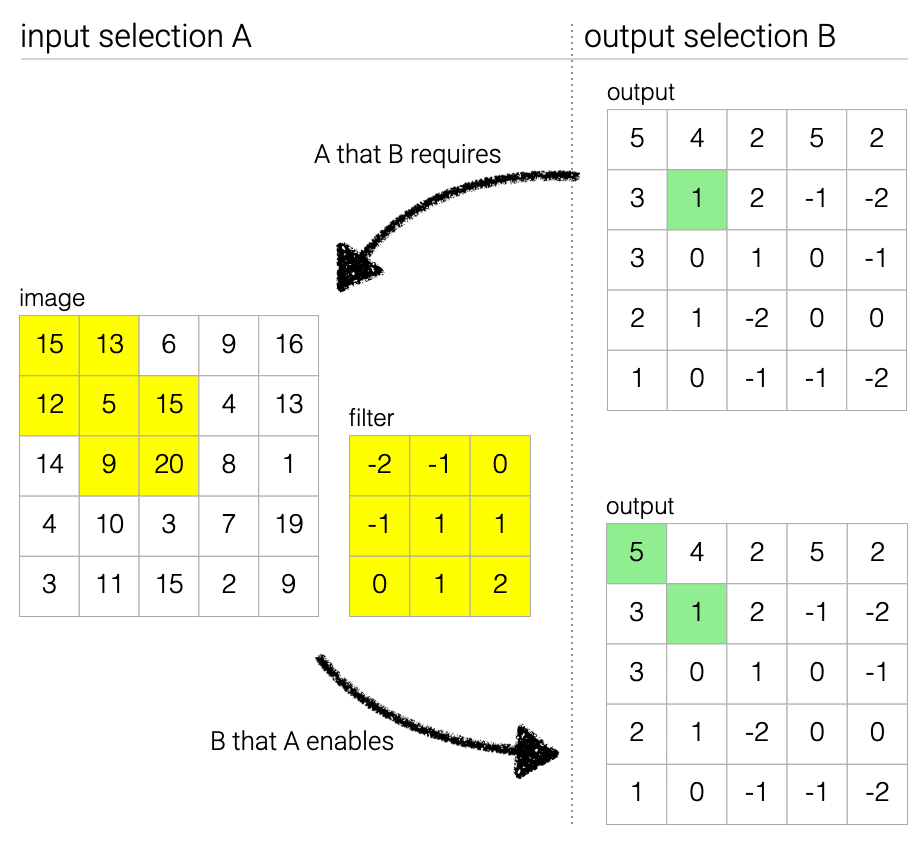
\includegraphics[scale=0.4]{fig/example/4-relations-1.png}}
      \vspace{2mm}
      \caption{Galois dependency $(\evalBwdF{T}, \evalFwdF{T})$}
      \label{fig:example:convolve-viz:galois-dependency}
   \end{subfigure}
   \begin{subfigure}{0.46\textwidth}
      {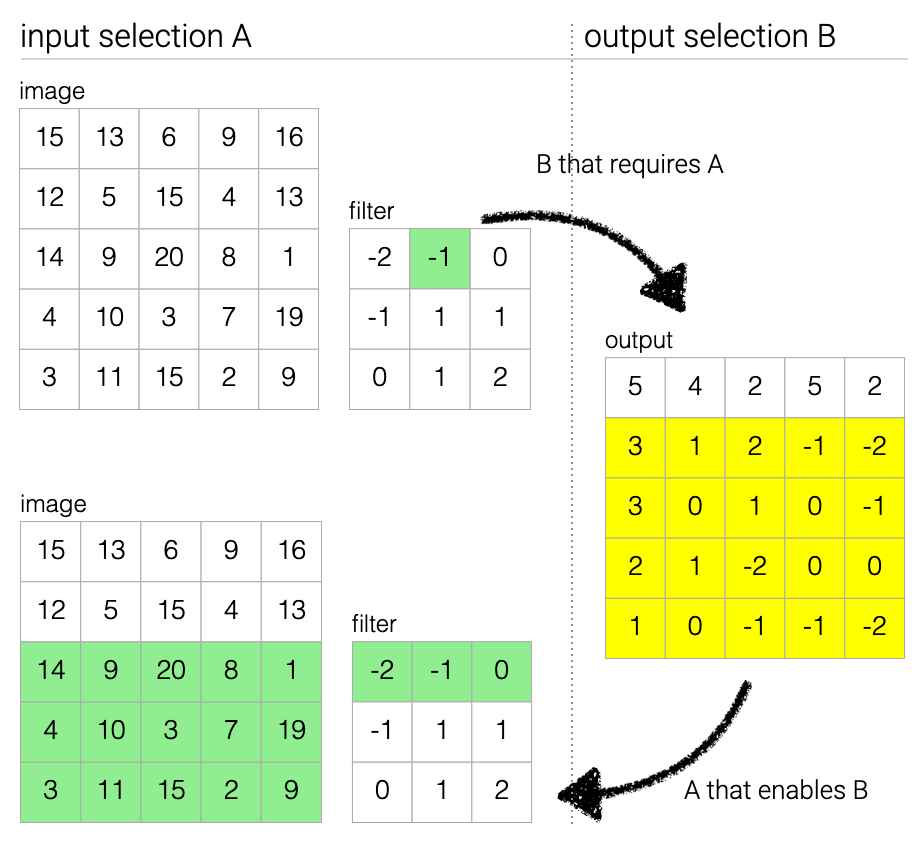
\includegraphics[scale=0.4]{fig/example/4-relations-2.png}}
      \vspace{2mm}
      \caption{De Morgan dual $(\dual{\evalFwdF{T}}, \dual{\evalBwdF{T}})$}
      \label{fig:example:convolve-viz:de-morgan-dual}
   \end{subfigure}
   \caption{Upper and lower pairs are dual; left and right pairs are adjoint}
   \label{fig:example:convolve-viz}
\end{figure}


\subsection{Towards a solution: Galois connections for data-linked visualisation}

Data visualisations are computed views of a data source. This suggests that it might be possible to adapt techniques from program analysis and data provenance to provide a runtime infrastructure that automatically supports linked selections. Then the data scientist or visualisation designer can concern themselves with cleaning, aggregating and presenting data, leaving the infrastructure to take care of linking visualisations to the underlying data sources and related visualisations to each other. This would be a step a data science which is more transparent by construction.

The fine-grained relationship between visual elements and data intuitively has the flavour of an adjunction. Given a data selection, we might ask whether it contains the data required to reconstruct --- whether it is \emph{sufficient for} --- a given part of the chart. Dually, given a visual selection, we might ask whether it is small enough to be generated by a given data selection. Additionally we might wonder whether there are minimal/maximal solutions to these problems.

These considerations points towards \emph{Galois connections} as a way of formalising these dynamic input-output relations, and indeed in the program slicing literature, dynamic analyses based on Galois connections have been developed for pure functional programs \cite{perera12a}, functional programs with effects \cite{ricciotti17}, and \piCalculus \cite{perera16d}. These ``Galois slicing'' techniques have the flavour of what we need, but are unable to compute the kind of sufficiency relation we just outlined. To see the problem, we briefly outline how Galois slicing works. The idea is generalise the notion of program and value to \emph{program slices} and \emph{value slices}, program and values where some subexpressions have been replaced by hole $\hole$. A program slice ``evaluates'' to a \emph{value slice}, a value where some subvalues have been replaced by $\hole$.

The problem with this approach is that it does not readily extend to a notion of ``selection'' where the part of the output (or input) of interest is not a prefix of the entire output (or input). For example, if we consider the following program, which has the value \lstinline{(0.25, 0.75)}:

\begin{figure}[H]
   \small
   \begin{subfigure}{0.32\textwidth}
      {\lstinputlisting[language=Fluid,escapeinside={(*@}{@*)}]{other-src/galois-slicing-1.example}}
   \caption{Wurble}
   \end{subfigure}
\end{figure}

\subsection{Linking cognate visualisations}

We use the term \emph{cognate} to describe visualisations that depend on common data. Intuitively, selections in cognate visualisations can be linked through their common data, which also a bidirectional quality: one must consider how dependencies flow ``backward'' from selections in one chart to the underlying data, and then ``forward'' from the selected data to a corresponding selection in the other chart. However the flavour of the forward dependency differs from the notion of ``sufficiency'' outlined in the previous section: to determine the related parts of the other chart, we must consider not what the data selection is \emph{sufficient} for, but what it is \emph{necessary} for: those parts of the other visualisation that

\begin{figure}[H]
   \small
   \lstinputlisting[language=Fluid]{fluid/convolution.fld.mod}
   \caption{Matrix convolution, with three methods for dealing with boundaries}
\end{figure}

\begin{figure}[H]
   \small
   \lstinputlisting[language=Fluid]{fluid/conv-extend.fld.mod}
   \caption{Convolving example matrix with supplied filter and choice of boundary method}
\end{figure}

